\documentclass[aspectratio=169,10pt]{beamer}

\usetheme[progressbar=frametitle]{metropolis}
\usepackage{appendixnumberbeamer}
\usepackage[utf8]{inputenc}
\usepackage{booktabs}
\usepackage[scale=2]{ccicons}
\usepackage{proof}
\usepackage{pgfplots}
\usepackage{fancyvrb}
\usepackage{stackengine}
\usepgfplotslibrary{dateplot}


\usepackage[T1]{fontenc}
\usepackage{color}
\usepackage{xcolor}
\definecolor{dkgreen}{rgb}{0,0.6,0}
\definecolor{gray}{rgb}{0.5,0.5,0.5}
\definecolor{mauve}{rgb}{0.58,0,0.82}

\usepackage{listings}
\lstset{%
  numberstyle=\tiny,
  numbersep=15pt,tabsize=4,
  flexiblecolumns=true,
  keywordstyle=\color{blue},
  commentstyle=\color{dkgreen},
  stringstyle=\color{mauve},
  numberstyle=\tiny\color{gray},
  language=Java,
  breaklines=true,
  breakatwhitespace=true,
  showstringspaces=false,
  aboveskip=1.2em,
  belowskip=1.2em,
  keywordstyle=\color{blue},
  keywordsprefix={@},
}

\usepackage{xspace}
\newcommand{\themename}{\textbf{\textsc{metropolis}}\xspace}

\title{Inferencia de facetas de declasificación}
\subtitle{Propuesta de solución}
% \date{\today}
\date{}
\author{Matías Meneses C.}
\institute{}
% \titlegraphic{\hfill
\includegraphics[height=1.5cm]{logo.pdf}}

\begin{document}

\maketitle

\begin{frame}{Índice de Contenidos}
  \setbeamertemplate{section in toc}[sections numbered]
  \tableofcontents[hideallsubsections]
\end{frame}

\section{Descripción del Problema}

\begin{frame}[fragile]{Descripción del Problema}
  Se quiere implementar una herramienta de inferencia de facetas públicas para un sistema de tipos de dos facetas, en el contexto de information flow control.
  \begin{itemize}
    \uncover<2->{\item El objetivo es facilitar el trabajo al programador, evitando que anote manualmente las anotaciones y cree las interfaces respectivas.}
    \uncover<3->{\item La faceta privada es dada.}
  \end{itemize}
\end{frame}

\section{Inferencia Global vs Inferencia Local}

\begin{frame}[fragile]{Inferencia Global vs Inferencia Local}

  \begin{onlyenv}<1>
		\only<2-|handout:0>{\stepcounter{framenumber}}
    La inferencia global es un problema no decidible, y la presencia de subtyping no mejora la situación.
    \begin{lstlisting}
    class Person {
      Person foo(Person a, Person b) {
        return a.bar(b);
      }

      Person bar(Person a) {
        return a.foo(a, this);
      }
    }
    \end{lstlisting}
  \end{onlyenv}
  \begin{onlyenv}<2>
    La inferencia global es un problema no decidible, y la presencia de subtyping no mejora la situación.
    \begin{lstlisting}
    class Person {
      @??? Person foo(@PersonBar Person a, @PersonFoo Person b) {
        return a.bar(b);
      }

      @??? Person bar(@PersonFoo Person a) {
        return a.foo(a, this);
      }
    }
    \end{lstlisting}
  \end{onlyenv}

  \begin{onlyenv}<3->
    Podemos realizar inferencia local, exigiendo que la firma de los métodos se encuentre completamente anotada.
  \end{onlyenv}
  \only<4>{Muy restrictivo!}

\end{frame}

\begin{frame}[fragile]{Inferencia Global Restringida}
  Si una expresión exterior al método actual tiene una faceta pública no definida, entonces no se generará ninguna constraint (por defecto es \textit{bottom}).
  \begin{onlyenv}<1>
		\only<2-|handout:0>{\stepcounter{framenumber}}
    \begin{lstlisting}
    class Person {
      Person foo(Person a, Person b) {
        return a.bar(b);
      }

      Person bar(Person a) {
        return a.foo(a, this);
      }
    }
    \end{lstlisting}
  \end{onlyenv}
  \begin{onlyenv}<2>
    \begin{lstlisting}
    class Person {
      @Person Person foo(@PersonBar Person a, @Person Person b) {
        return a.bar(b);
      }

      @Person Person bar(@PersonFoo Person a) {
        return a.foo(a, this);
      }
    }
    \end{lstlisting}
  \end{onlyenv}
    \begin{onlyenv}<3>
    \begin{lstlisting}
    class Person {
      @Person Person foo(@PersonBar Person a, @PersonFoo Person b) {
        return a.bar(b);
      }

      @Person Person bar(@PersonFoo Person a) {
        return a.foo(a, this);
      }
    }
    \end{lstlisting}
  \end{onlyenv}
\end{frame}

\section{Propuesta: Proceso iterativo de inferencia asistida}
\begin{frame}[fragile]{Propuesta: Proceso iterativo de inferencia asistida}
  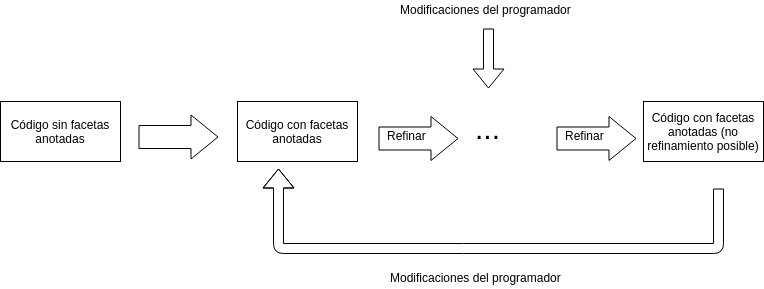
\includegraphics[width=1.0\textwidth]{img/diagrama.png}
\end{frame}
\begin{frame}[fragile]{Propuesta: Proceso iterativo de inferencia asistida}

    \begin{columns}
      \begin{column}{0.5\textwidth}
				\begin{onlyenv}<1-2>
					\only<2-|handout:0>{\stepcounter{framenumber}}
    \begin{lstlisting}
class Person {
  void foo(Person a, Person b) {
    a.bar(b);
  }

  void bar(Person p) {
    p.baz(p);
  }

  void baz(Person p) {
    print(p);
  }
}
\end{lstlisting}
\end{onlyenv}
\begin{onlyenv}<3-4>
\begin{lstlisting}
class Person {
  @void void foo(@PersonBar Person a, @Person Person b) {
    a.bar(b);
  }

  @void void bar(@PersonBaz Person p) {
    p.baz(p);
  }

  @void void baz(@Person Person p) {
    print(p);
  }
}
\end{lstlisting}
\end{onlyenv}
\begin{onlyenv}<5-6>
\begin{lstlisting}
class Person {
  @void void foo(@PersonBar Person a, @PersonBaz Person b) {
    a.bar(b);
  }

  @void void bar(@Person Person p) {
    p.baz(p);
  }

  @void void baz(@Person Person p) {
    print(p);
  }
}
\end{lstlisting}
\end{onlyenv}
\begin{onlyenv}<7>
\begin{lstlisting}
class Person {
  @void void foo(@PersonBar Person a, @Person Person b) {
    a.bar(b);
  }

  @void void bar(@Person Person p) {
    p.baz(p);
  }

  @void void baz(@Person Person p) {
    print(p);
  }
}
\end{lstlisting}
\end{onlyenv}
      \end{column}

      \begin{column}{0.5\textwidth}  %%<--- here
				\begin{onlyenv}<2>
          
\includegraphics[height=\fontcharht\font`\B*3]{img/bulb.png}
					\colorbox{red!30}{Inferir facetas no definidas.}
			\end{onlyenv}
			\begin{onlyenv}<4,6>
				
\includegraphics[height=\fontcharht\font`\B*3]{img/bulb.png}
				\colorbox{red!30}{Flujo no permitido. Refinar facetas.}
		\end{onlyenv}
		\begin{onlyenv}<7>
			\colorbox{green!30}{No hay errores :)}
	\end{onlyenv}
      \end{column}
    \end{columns}



\end{frame}

\begin{frame}[fragile]{Propuesta: Formalización}
  Se extiende el lenguaje base de Type-based relaxed noninterference para adaptarlo a las necesidades y sintaxis de un subconjunto de Dart, incluyendo referencias, instrucciones condicionales y secuencias de instrucciones.
  \begin{onlyenv}<1>
    \only<2-|handout:0>{\stepcounter{framenumber}}
    \begin{Verbatim}[fontsize=\small]
  e ::= v | e.m(e) | x
  v ::= [z: U => list(m(x)e)]
T,U ::= O | TVar
  O ::= Obj(TVar). [list(m: S -> S)]
  S ::= T < U

  x variable
  m method label
  S security type
  U public facet, T private facet
\end{Verbatim}
  \end{onlyenv}
    \begin{onlyenv}<2>
    \begin{Verbatim}[fontsize=\small]
  e ::= v | e.m(e) | x | e;e | e = e | if e then e else e |
        while e do e | m(x)e
  v ::= [z: U => list(m(x)e)] | DV
  U ::= O | TVar | void
  O ::= Obj(TVar). [list(m: U -> U)]

  x variable
  m method label
  U public facet
  DV Dart primitive value
\end{Verbatim}
  \end{onlyenv}
\end{frame}

\begin{frame}[fragile]{Propuesta: Formalización}
  \begin{onlyenv}<1->
    \only<2-|handout:0>{\stepcounter{framenumber}}
    Se escriben las reglas de inferencia, que generan un set de constraints a resolver.
  \end{onlyenv}
  \begin{onlyenv}<2>
    \begin{center}
      (seq)
      \[\infer{\Gamma, M, pc, pt2 \vdash e1;e2 : t2\, |\, C2 \cup C1}{\Gamma, M, pc, pt1 \vdash e1 : t1\, |\, C1 \qquad \Gamma, M, pc, pt2 \vdash e2 : t2\, |\, C2}\]
    \end{center}

  \end{onlyenv}

  \begin{onlyenv}<3>
    \begin{center}
      (method)
      \[\infer{\Gamma, M, pc, pt \vdash m(x)e : t3\, |\, \{t3 <: t2\} \cup C2 \cup C1}{\Gamma, M, pc, pt1 \vdash m : t1 \rightarrow t2\, |\, C1 \qquad \Gamma, M, pc, pt2 \vdash e : t3\, |\, C2}\]
    \end{center}

  \end{onlyenv}

  \begin{onlyenv}<4>
    \begin{center}
      (assn)
      \[\infer{\Gamma, M, pc, pt \vdash e1 = e2 : void\, |\, \{t2 <: t1\} \cup \{pc <: t1\} \cup C2 \cup C1}{\Gamma, M, pc, pt1 \vdash e1 : t1\, |\, C1 \qquad \Gamma, M, pc, pt2 \vdash e2 : t2\, |\, C2}\]
    \end{center}
  \end{onlyenv}

  \begin{onlyenv}<5>
    \begin{center}
      (if)
      \[\infer{\Gamma, M, pc, pt \vdash \text{if e1 then e2 else e3} : t\, |\, \{t2 <: t\} \cup \{t3 <: t\} \cup C3 \cup C2 \cup \{t1 <: pc1\} \cup C1}{\stackanchor{$\Gamma, M, pc, pt1 \vdash e1 : t1\, |\, C1$}{\stackanchor{$\Gamma, M, pc1, pt2 \vdash e2 : t2\, |\, C2$}{$\Gamma, M, pc1, pt3 \vdash e3 : t3\, |\, C3$}}}\]
    \end{center}
  \end{onlyenv}

  \begin{onlyenv}<6>
    \begin{center}
      (call)
      \[\infer{\Gamma, M, pc, pt \vdash e1.m(e2) : t4\, |\, \{t2 <: t3\} \cup \{t1 <: [[m: t3 \rightarrow t4]]\} \cup C2 \cup C1}{\Gamma, M, pc, pt1 \vdash e1 : Obj(t1). [[m : t3 \rightarrow t4]]\, |\, C1 \qquad \Gamma, M, pc, pt2 \vdash e2 : t2\, |\, C2}\]
    \end{center}
  \end{onlyenv}
\end{frame}

\section{Resolución de Constraints}
\begin{frame}[fragile]{Resolución de Constraints}
  Para resolver las constraints se usan los operadores \texttt{join} ($\lor$) y \texttt{meet} ($\land$) en la lattice que forman las facetas de declasificación.
  \begin{itemize}
    \item{$\{t1 <: t2\}, \{t1 <: t3\} \implies \{t1 <: t2 \land t3 \} $}
    \item{$\{t2 <: t1\}, \{t3 <: t1\} \implies \{t2 \lor t3 <: t1\} $}
  \end{itemize}
\end{frame}

{\setbeamercolor{palette primary}{fg=black, bg=yellow}
\begin{frame}[standout]
  
\end{frame}
}

\appendix

\begin{frame}[fragile]{Backup slides}
  Sometimes, it is useful to add slides at the end of your presentation to
  refer to during audience questions.

  The best way to do this is to include the \verb|appendixnumberbeamer|
  package in your preamble and call \verb|\appendix| before your backup slides.

  \themename will automatically turn off slide numbering and progress bars for
  slides in the appendix.
\end{frame}

\begin{frame}[allowframebreaks]{References}

  \bibliography{defensa}
  \bibliographystyle{abbrv}

\end{frame}

\end{document}
